\section{Experimental Results}

\label{sec:results}

\paragraph{The implementation}
We have implemented Angluin's learning algorithm, closely following the
high-level description in \cite{Angluin:regset}. Furthermore, we have
implemented our proposed optimization for prefix-closed models. It
differs from the ordinary learner only in that it can infer the answer
of some membership queries, due to properties of prefix-closed
languages. Accordingly, the number of membership queries can be
expected to be smaller, while the number of equivalence queries is
unchanged. Furthermore, it requires the same amount of memory for the
observation table.

We simulated the teacher (and oracle) on the same computer as the learner, for
reasons of simplicity. In practice, a teacher will typically be
realized as a process communicating with a slow external device.

Our learners are written in Java using the library AMoRE
developed at RWTH Aachen for maintaining automata.

\paragraph{The experiments} 
Our experiments aim at finding out how our implementation of Angluin's
learner and our optimized learner perform and scale in practice. We
have examined real-world examples and randomly generated examples. 
The real-world examples are several protocols shipped with the
Edinburgh Concurrency Workbench. They were originally formulated in
Milner's CCS. We transformed their transition system representation
into minimized prefix-closed DFA.

For reasons of comparison, we studied two kinds of random examples,
prefix-closed random examples and arbitrary random DFA.

As pointed out before, the expected bottle-neck in practice for a
learner is the number of membership and equivalence queries, since a
communication with a typically slow external device is required and
quite many queries are needed. Thus, we concentrated our experiments
on the number of membership and equivalence queries. To get an overall
picture, we also measured the execution time and memory consumption
for large examples. Hereby ``execution time'' means the total
execution time minus the time for equivalence queries. In other words,
we measure the time spent by the learner plus the one spent by the
teacher. Since there are several ways to realize The oracle, we
disregard this time.

In our experiments, we vary the alphabet size and the number of states
of the automata. Our measurements do not adhere to strong statistical
requirements. Thus, they cannot be used to \emph{prove} the practical
performance of the algorithms in a statistical sense. However, they
are good enough to show a tendency and to point out directions for
future optimizations and analysis.


\subsection{Angluin's algorithm}

A theoretical upper bound for the number of membership queries is the
worst-case size of the observation table. In, 
\cite{Angluin:regset}, Angluin calculates this bound to
$O(m|\alphabet||\states|^2)$, where $m$ is the maximum length of any
received counterexample. If the $Oracle$ always provides a smallest
counterexample, then $m = |\states|$, and thus the number of
membership queries are in the worst case $O(|\alphabet|{|\states|}^3)$.

To investigate how the algorithm behaves in practice, we studied it on
arbitrary random examples as well as prefix-closed random
examples. Let us start with the arbitrary ones.

\subsubsection{Random examples}

\paragraph{The samples}
We studied random examples varying the number of states and letters.
We generated and learned DFA between 10 and 100 states, in steps of 10. 

Each set of measurements was carried out with different alphabet size.
For systems with up to 60 states, we studied from 5 up to 50 letters
in steps of 5, and, for systems with more states, from 10 up to 50
letters in steps of 10.

We sampled 10 DFA for each state and letter combination, except for
those with the number of states 70 or higher, for which we sampled
only 5.

\paragraph{Experiences}
Fixing the number of states but varying the number of letters, we
observe a linear behavior, as expected. See
Figure~\ref{fig:pic_letter}, in which the number of states are fixed
to 10 and 60.

The collected data shows that, in terms of membership queries,
Angluin's learning algorithm is approximately linear in states on
random DFA, despite the algorithm's worst-case complexity. As an
example, we show the number of membership queries relative to the
number of states, with the number of letters fixed to 10 and 40, in
Figure~\ref{fig:pic}.

\begin{figure}
  \begin{center}
        \epsfig{file=pic_letter.ps, height=9.5cm,angle=270}
    \caption{Random automata, number of states fixed to 10 and 60.\label{fig:pic_letter}}
  \end{center}
\end{figure}


\begin{figure}
  \begin{center} \epsfig{file=pic.ps, height=9.5cm,angle=270}
  \caption{Random automata, number of letters fixed to 10 and
  40.\label{fig:pic}} \end{center}
\end{figure}

To get an impression of the performance of the algorithm, learning a
random example of 100 states and 25 letters, took 1 hour, 40,000
membership and 15 equivalence queries, and 110 MB of space. This long
execution time was one reason for learning fewer automata of larger
sizes. The other reason is the huge memory consumption of the
observation table.

Additionally, we studied the number of membership queries with respect
to the number of transitions, $|\transf| = |\states||\alphabet|$. This
is possible since we discovered by our measurements that the nominal
variables states and letters behave interchangeably. At the very
bottom in Figure~\ref{fig:games_talk} is the curve that shows the
number of membership queries with respect to the number of
transitions. We can describe the observations roughly by the relation
$|membership~ queries| = k |\transf|$, where $k \approx 14$.

\begin{figure}
  \begin{center}
	\epsfig{file=games_talk.ps, height=9.5cm,angle=270}
    \caption{Membership queries with respect to transitions.\label{fig:games_talk}}
  \end{center}
\end{figure}

\subsubsection{Random prefix-closed examples}

\paragraph{The samples}
In general, prefix-closed DFA require more time and space to learn
with Angluin's algorithm, so we studied fewer samples. We learned
automata with 10 to 50 states in steps of 10 and varied the number of
letters from 10 to 50 in steps of 10. We learned approximately 10
automata of each kind up to 30 states and fewer of larger ones.

\paragraph{Experiences}
As mentioned before, arbitrary random examples are in general easier
to learn than prefix-closed random examples. An example for this is
shown in Figure~\ref{fig:pic_randomPrefixClosed_single}. Learning a
particular random generated automaton, with 40 letters and 40 states, requires
approximately 19,000 membership queries and a prefix-closed automaton
of the same size requires 40,000 membership queries, that is about
twice as many.

\begin{figure}
  \begin{center}
        \epsfig{file=pic_randomPrefixClosed_single.ps, height=9.5cm,angle=270}
    \caption{Random prefix-closed automata and random automata, both with
40 letters.\label{fig:pic_randomPrefixClosed_single}}
  \end{center}
\end{figure}

Let us study the cause for this difference. Angluin's learning
algorithm tries to learn an automaton by finding representatives of
different Nerode's right congruence classes, as described in
Section~\ref{sec:angluin:direct}. To show that two strings $u$ and $v$
are not members of the same congruence class, it has to find one
string $w$ so that $uw$ is accepted but $vw$ not, or the other way
around. In minimal prefix-closed DFA, as maintained by Angluin, every
state except one is accepting, and it is more likely that states
accept almost the same language. This makes it more difficult to find
a distinguishing string $w$.

Furthermore, we see that the curves for learning prefix-closed
languages grow steeper than for arbitrary random examples. On
prefix-closed examples we come closer to the worst case complexity of
Angluin's algorithm. Thus, prefix-closed examples are harder to learn
than arbitrary ones. This result is slightly disappointing, since
reactive systems can usually be modeled by prefix-closed automata.
This experience is in contrast to the one gained in the area of model
checking, where worst-case complexities usually do not show up in
real-world examples.

A particular random example with 100 states and 25 letters took 11
hours, 110,000 membership queries, 29 equivalence queries and 160 MB
of memory.

The top curve in Figure~\ref{fig:games_talk} shows
membership queries versus transitions for random prefix-closed
examples. It is no longer linear. A very rough description
of the observations is given by the quadratic relation $|\mq| = k
{|\transf|}^2$, where $k \approx 0.016$.

\subsection{The optimization for prefix-closed systems}

As pointed out in the previous section, the optimized version for
prefix-closed languages takes into account that extensions of rejected
strings are rejected. Before issuing a membership query to the
teacher, we check whether we can deduce it from previous membership
queries. In our setting, the optimized learner gives about the same
execution time as the ordinary learner. Since we simulate the \Teacher
on the same computer, a query takes roughly the same amount of time as
a table lookup. Note that in the setting where a concrete hardware
system is learned, the time for a table lookup might be negligible
compared to the time a membership query needs.

\subsubsection{Random prefix-closed examples}

\paragraph{The samples}
On the optimized learner, we studied the same random prefix-closed examples as with the ordinary learner.

\paragraph{Experiences}

We observe that the optimization yields noteworthy savings in terms
of membership queries. To give an example, we have shown the number of
membership queries with respect to the number of states in
Figure~\ref{fig:pic_randomPrefixClosed} and Figure~\ref{fig:pic_randomPrefixClosed_big} for the number of letters
fixed to 10 and 40, for the optimized version in comparison with
Angluin's version. We save in case of larger automata approximately
20\% in both cases when using the optimization.

The particular example of size 100 states and 25 letters, from the
previous subsection, took 12 hours, 96,000 membership queries, 29
equivalence queries and 160 MB of memory for our optimized learner.

The middle curve in Figure~\ref{fig:games_talk} shows
membership queries with the optimized learner versus transitions for
random prefix-closed examples. A very rough summary of our
observations is $|\mq| = k {|\transf|}^2$, with $k \approx 0.013$.

\begin{figure}
  \begin{center}
        \epsfig{file=pic_randomPrefixClosed.ps, height=9.5cm,angle=270}
    \caption{Random prefix-closed examples learned with Angluin and optimization, number of letters fixed to 10.\label{fig:pic_randomPrefixClosed}}
  \end{center}
\end{figure}


\begin{figure}
  \begin{center}
        \epsfig{file=pic_randomPrefixClosed_big.ps, height=9.5cm,angle=270}
    \caption{Random prefix-closed examples learned with Angluin and
    optimization, number of letters fixed to 40.\label{fig:pic_randomPrefixClosed_big}}
  \end{center}
\end{figure}

\subsubsection{Real-world examples}

\paragraph{The samples} We studied 6 transition systems of CCS
processes. They are simple examples like buffers, vending machines, or
several examples of schedulers and mutual exclusion protocols. Their
number of states lie between 2 and 13 and the number of letters
between 3 and 6. Note that we learned minimized DFA representations of
the given protocols.

We failed to learn some larger protocols, namely some instances of
parameterized schedulers, the Jobshop (77 states, 7 letters) and an
ATM protocol (1715 states, 27 letters). The reason is that we did not
invest effort into a good algorithm for finding counterexamples; it
took too long to find counterexamples for the protocols in question.
(Note that the execution time which we measure is independent of the
time spent for finding counterexamples.) The ATM, though, failed due
to lack of memory.

\paragraph{Experiences}

The number of membership and equivalence queries, as well as execution
time, are shown in Table~\ref{table:realworld_ex}.\footnote{In all
tables {\it mq} is an abbreviation of the number of membership
queries, {\it eq} of the number of equivalence queries and {\it opt}
of the optimization for prefix-closed systems.}

\begin{table}[h]\footnotesize
\begin{center}
\begin{tabular}{|r|r|r|r|r|r|r|r|r|r|r|}
\hline 
Protocol & states & letters & \parbox{1cm}{\mqtable} &
\parbox{1cm}{\eqtable} & \parbox{1cm}{\ettable (ms)} & 
\parbox{1cm}{\mqtable with opt} & \parbox{1cm}{\eqtable with opt} &
\parbox{1cm}{\ettable with opt (ms)}\\
\hline 
Abp-lossy & 3 & 3 & 22 & 2 & 65 & 9 & 2 & 1057\\
Buff3 & 9 & 3 & 202 & 5 & 2305 & 77 & 5 & 4907\\
Dekker-2 & 2 & 3 & 7 & 1 & 646 & 4 & 1 & 7\\
Peterson-2 & 2 & 3 & 7 & 1 & 352 & 4 & 1 & 288\\
Sched2 & 13 & 6 & 691 & 7 & 43031 & 115 & 7 & 48207\\
VMnew & 11 & 4 & 513 & 7 & 26191 & 191 & 7 & 20091\\
\hline 
\end{tabular}
\end{center}
\caption{Learning real-world examples.\label{table:realworld_ex}}
\end{table}

Comparing the number of membership queries of the optimized version
with respect to Angluin's algorithm, we saved about 60\%. Details
can be found in Table~\ref{table:realworld_savings}.

\begin{table}[h]\footnotesize
  \begin{center}
\begin{tabular}{|r|r|r|r|}
\hline 
Protocol & \parbox{1.5cm}{\mqtable} &
\parbox{1.5cm}{\mqtable with opt} & \parbox{1.5cm}{saved \mqtable (\%)} \\
\hline 
Abp-lossy & 22 & 9 & 59\\
Buff3 & 202 & 77 & 62\\
Dekker-2 & 7 & 4 & 43\\
Peterson-2 & 7 & 4 & 43\\
Sched2 & 691 & 115 & 83\\
VMnew & 513 & 191 & 63\\
\hline 
\end{tabular}
\end{center}
\caption{Saved membership queries with optimization.\label{table:realworld_savings}}
\end{table}

To check whether real-world examples show a different behavior in
learning by the optimized algorithm, we compared them with random
prefix-closed examples of the same sizes. Each result is an average
over 6 to 8 fixed size random samples. The results are
shown in Table~\ref{table:random_ex}.

\begin{table}[h]\footnotesize
  \begin{center}
\begin{tabular}{|r|r|r|r|r|r|r|r|}
\hline 
states & letters & \parbox{1.0cm}{\mqtable} & \parbox{1.0cm}{
\eqtable} & \parbox{1.0cm}{\ettable (ms)} &
\parbox{1.0cm}{\mqtable with opt} & \parbox{1.0cm}{\eqtable with opt (ms)} &
\parbox{1.0cm}{\ettable with opt (ms)}\\
\hline 
3 & 3 & 22 & 2 & 153 & 12 & 2 & 115\\
9 & 3 & 233 & 5 & 1443 & 173 & 5 & 1384\\
2 & 3 & 7 & 1 & 25 & 4 & 1 & 10\\
13 & 6 & 992 & 8 & 10885 & 737 & 8 & 10989\\
11 & 4 & 497 & 7 & 5230 & 341 & 7 & 5408\\
\hline 
\end{tabular}
\end{center}
\caption{Random prefix-closed automata.\label{table:random_ex}}
\end{table}

We see that the optimized learner is often better on the protocols
relative to random examples (see
Table~\ref{table:compare_ex_rand}). On average the real-world examples
required 7\% fewer membership queries without and 35\% with the optimization. This
might indicate that real-world examples exhibit a certain structure
which makes the algorithm perform better.

\begin{table}[h]\footnotesize
  \begin{center}
\begin{tabular}{|r|r|r|}
\hline 
protocol & \parbox{1.5cm}{mq quotient} &
\parbox{1.5cm}{with opt}\\

\hline 
Abp-lossy & 1 & 0.75\\
Buff3 & 0.87 & 0.45\\
Dekker-2 & 1 & 1\\
Peterson-2 & 1 & 1\\
Sched2 & 0.70 & 0.16\\
VMnew & 1.03 & 0.56\\
\hline 
\end{tabular}
\end{center}
\caption{Random prefix-closed automata vs. real-world examples.\label{table:compare_ex_rand}}
\end{table}

%%% Local Variables: 
%%% mode: latex
%%% TeX-master: "main"
%%% TeX-master: "main"
%%% End: 
% LocalWords:  Angluins
